

%%%%%%%%%%%%%%%%%%%%%%%%%%%%%%%%%%%55%%
\begin{frame} [plain]
    \frametitle{}
    \Background[1] 
    \begin{center}
    {\huge 第7讲:量子算法(3)    }
    \end{center}  
    \addtocounter{framenumber}{-1}   
\end{frame}
%%%%%%%%%%%%%%%%%%%%%%%%%%%%%%%%%%

\section{1.相位估计}

\begin{frame}
    \frametitle{相位估计}
    \begin{itemize}
        \Item 量子傅里叶变换是相位估计的关键
        \Item 相位估计是许多量子算法的基础
        \Item 比如:求本征值,大数质因式分解
    \end{itemize}
\end{frame}

\begin{frame}
    \frametitle{相位估计的目的}
    \begin{itemize}
        \Item 酉变换与薛定谔方程等价
        \[ i\hbar \frac{d\rs{\Psi}}{dt}=H \rs{\Psi}\]
        \[\rs{\Psi'}=U\rs{\Psi}\]
        \[\rs{\Psi(t_2)} =U(t_1,t_2) \rs{\Psi(t_2)}\]
        \[U(t_1,t_2) = exp[\frac{-iH(t_2-t_1)}{\hbar}]\]
        \Item 设U有本征矢$\rs{u}$,对应本征值为 $exp(2\pi i \varphi)$
        \Item 相位估计的目的是求$\varphi$
    \end{itemize}
\end{frame}

\begin{frame}
    \frametitle{相位估计三步走}
    \begin{enumerate}
        \item 混合:把$\rs{u}$的相位$\varphi$与t个叠加态混合成傅里叶乘积式
        \item 反傳里叶变换得到$\varphi_1 \varphi_1 \cdots\varphi_t$
        \item 测量得到 $\varphi$
    \end{enumerate}
\end{frame}

\begin{frame}
    \frametitle{混合量子线路}
    \tikzstyle{every picture}+=[remember picture]
    \begin{figure}
      \centerline{
        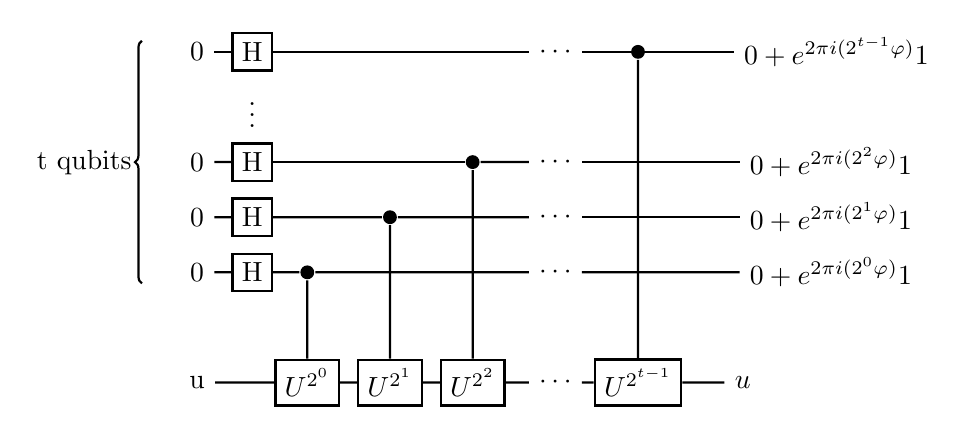
\begin{tikzpicture}[thick,scale=0.7]
        %
        % `operator' will only be used by Hadamard (H) gates here.
        % `phase' is used for controlled phase gates (dots).
        % `surround' is used for the background box.
        \tikzstyle{H} = [draw,fill=white,minimum size=1.2em] 
        \tikzstyle{U} = [draw,fill=white,minimum size=1.3em] 
        \tikzstyle{D} = [fill,shape=circle,minimum size=5pt,inner sep=0pt]
        %\tikzstyle{surround} = [fill=blue!10,thick,draw=black,rounded corners=2mm]
        
        % Bracket
        \draw[decorate,decoration={brace},thick] (-1,-4.2) -- node[left] {t qubits} (-1, 0.2);
        %\draw[decorate,decoration={brace},thick] (-1,-6.6) -- (-1, -5.4);

        % Column 0
        \node at (0,0)  (Q00) {\rs{0}}; 
        
        \node at (0,-2) (Q02) {\rs{0}}; 
        \node at (0,-3) (Q03) {\rs{0}}; 
        \node at (0,-4) (Q04) {\rs{0}}; 

        \node at (0,-6) (Q06) {\rs{u}}; 
        
 %      % Column 1
        \node[H] (H10) at (1,0) {H} edge [-] (Q00);
        \node    (D11) at (1,-1) {$\vdots $} ;
        \node[H] (H12) at (1,-2) {H} edge [-] (Q02);
        \node[H] (H13) at (1,-3) {H} edge [-] (Q03);
        \node[H] (H14) at (1,-4) {H} edge [-] (Q04);
 %
 %      % Column 2
        \node[D] (D24) at (2,-4) {} edge [-] (H14);
        \node[U] (U26) at (2,-6) {$U^{2^0}$} edge [-] (Q06);
        \draw[-] (D24) -- (U26);

 %
 %      % Column 3.5
        \node[D] (D33) at (3.5,-3) {} edge [-] (H13);
        \node[U] (U36) at (3.5,-6) {$U^{2^1}$} edge [-] (U26);
        \draw[-] (D33) -- (U36);

  %     % Column 5
        \node[D] (D52) at (5,-2) {} edge [-] (H12);
        \node[U] (U56) at (5,-6) {$U^{2^2}$} edge [-] (U36);
        \draw[-] (D52) -- (U56);%

        % Column 6.5

        \node (D60) at (6.5,0) {$\cdots$} edge [-] (H10);

        \node (D62) at (6.5,-2) {$\cdots$} edge [-] (D52);
        \node (D63) at (6.5,-3) {$\cdots$} edge [-] (D33);
        \node (D64) at (6.5,-4) {$\cdots$} edge [-] (D24);

        \node (D66) at (6.5,-6) {$\cdots$} edge [-] (U56);

        % Column 8 
        \node[D] (D80) at (8,0) {} edge [-] (D60);
        \node[U] (U86) at (8,-6) {$U^{2^{t-1}}$} edge [-] (D66);
        \draw[-] (D80) -- (U86);%
 
 %      % Column 9.5
        \node at (11.6,0)  (H90) {$\rs{0}+e^{2\pi i (2^{t-1} \varphi)} \rs{1}$} edge [-] (D60); 

        \node at (11.5,-2) (H92) {$\rs{0}+e^{2\pi i (2^{2} \varphi)} \rs{1}$} edge [-] (D62);  
        \node at (11.5,-3) (H93) {$\rs{0}+e^{2\pi i (2^{1} \varphi)} \rs{1}$} edge [-] (D63);  

        \node at (11.5,-4) (H94) {$\rs{0}+e^{2\pi i (2^{0} \varphi)} \rs{1}$} edge [-] (D64);  

        \node at (9.9,-6) (H96) {$\rs{u}$} edge [-] (U86);    

    \end{tikzpicture}
    }
    \end{figure}
\end{frame}

\begin{frame}
    {\Bullet}~受控U门的做作用效果, 作用到本征态$\rs{u}$,得到本征值 $e^{2\pi i \varphi}$ 
    \begin{itemize}
        \item $\rs{0}U\rs{u}=\rs{0}\rs{u}$
        \item $\rs{1}U\rs{u}=\rs{1} e^{2\pi i \varphi}\rs{u}$ 
    \end{itemize}
    {\Bullet}~线路工作原理 \\
    \begin{itemize}
        \item $H\rs{0}=\Pstate$
        \item $\Pstate U\rs{u}=\dfrac{1}{\sqrt{2}} (\rs{0}\rs{u} +  e^{2\pi i \varphi}\rs{1}\rs{u})= \dfrac{1}{\sqrt{2}} (\rs{0} +  e^{2\pi i \varphi}\rs{1})\rs{u} $ 
        \item $\Pstate U^{2^n}\rs{u}= \dfrac{1}{\sqrt{2}} (\rs{0} + e^{2\pi i (2^n \varphi)\rs{1} })\rs{u} $ 
    \end{itemize}
\end{frame}

\begin{frame}
    \frametitle{}
    {\Bullet}~混合之后,t-qubits为:
    \[ \dfrac{1}{\sqrt{2^t}} [\rs{0} + e^{2\pi i (2^{t-1} \varphi)\rs{1} }] [\rs{0} + e^{2\pi i (2^{t-2} \varphi)\rs{1} }]\cdots [\rs{0} + e^{2\pi i (2^0 \varphi)\rs{1} }] \]
    考虑到$\varphi$的二进制形式:
    \[\varphi=0.\varphi_1 \varphi_2 \cdots \varphi_t = \frac{\varphi_1}{2^1} + \frac{\varphi_2}{2^2}+\cdots + \frac{\varphi_t}{2^t}\]
    \[2^{t-1} \varphi= \varphi_1 \varphi_2 \cdots \varphi_{t-1}.\varphi_t=0.\varphi_t\]
    \[2^{t-2} \varphi= \varphi_1 \varphi_2 \cdots \varphi_{t-2}.\varphi_{t-1}\varphi_t=0.\varphi_{t-1}\varphi_t\]
    上式可写成
    \[ \dfrac{1}{\sqrt{2^t}} [\rs{0} + e^{2\pi i 0.\varphi_t)}\rs{1} ] [\rs{0} + e^{2\pi i 0.\varphi_{t-1}\varphi_t }\rs{1} ]\cdots [\rs{0} + e^{2\pi i 0.\varphi_1\varphi_2\cdots \varphi_t}\rs{1}] \]
    正是傅里叶变换乘积式! 
\end{frame}

\begin{frame}
    \frametitle{傅里叶反变换}
    以三量子比特线路为例:
    \tikzstyle{every picture}+=[remember picture]
    \begin{figure}
      \centerline{
        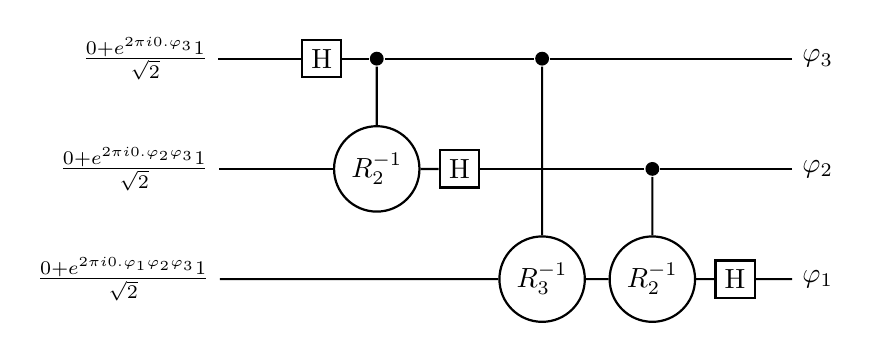
\begin{tikzpicture}[thick,scale=0.7]
        %
        % `operator' will only be used by Hadamard (H) gates here.
        % `phase' is used for controlled phase gates (dots).
        % `surround' is used for the background box.
        \tikzstyle{H} = [draw,fill=white,minimum size=1.2em] 
        \tikzstyle{U} = [draw,shape=circle,fill=white,minimum size=1.2em] 
        \tikzstyle{D} = [fill,shape=circle,minimum size=5pt,inner sep=0pt]
        %\tikzstyle{surround} = [fill=blue!10,thick,draw=black,rounded corners=2mm]
        
        % Bracket
        %\draw[decorate,decoration={brace},thick] (-1,-4.2) -- node[left] {t qubits} (-1, 0.2);
        %\draw[decorate,decoration={brace},thick] (-1,-6.6) -- (-1, -5.4);

        % Column 0
        \node at (-2.2,0)  (Q00) {$\frac{\rs{0}+e^{2\pi i 0.\varphi_3}\rs{1}}{\sqrt{2}}$}; 
        \node at (-2.4,-2) (Q01) {$\frac{\rs{0}+e^{2\pi i 0.\varphi_2\varphi_3}\rs{1}}{\sqrt{2}}$}; 
        \node at (-2.6,-4) (Q02) {$\frac{\rs{0}+e^{2\pi i 0.\varphi_1\varphi_2\varphi_3}\rs{1}}{\sqrt{2}}$}; 
        
 %      % Column 1
        \node[H] (H10) at (1,0) {H} edge [-] (Q00);
 %
 %      % Column 2
        \node[D] (D20) at (2,0) {} edge [-] (H10);
        \node[U] (U21) at (2,-2) {$R_2 ^{-1}$} edge [-] (Q01);
        \draw[-] (D20) -- (U21);

 %
 %      % Column 3.5
        \node[H] (H31) at (3.5,-2) {H} edge [-] (U21);

  %     % Column 5
        \node[D] (D50) at (5,0) {} edge [-] (D20);
        \node[U] (U52) at (5,-4) {$R_3 ^{-1}$} edge [-] (Q02);
        \draw[-] (U52) -- (D50);%

        % Column 6.5

        \node[D] (D61) at (7,-2) {} edge [-] (H31);
        \node[U] (U62) at (7,-4) {$R_2 ^{-1}$} edge [-] (U52);
        \draw[-] (D61) -- (U62);%

        % Column 8 
        \node[H] (H82) at (8.5,-4) {H} edge [-] (U62);

 
 %      % Column 9.5
        \node at (10,0)  (Q90) {$\rs{\varphi_3}$} edge [-] (D50); 
        \node at (10,-2)  (Q91) {$\rs{\varphi_2}$} edge [-] (D61);  
        \node at (10,-4)  (Q92) {$\rs{\varphi_1}$} edge [-] (H82); 
    \end{tikzpicture}
    }
    \end{figure}
\end{frame}


\begin{frame}
    \frametitle{推导}
    {\Bullet}~第一个量子比特过H门
    \begin{itemize}
        \item $\varphi_3=0; \quad \frac{\rs{0}+e^{2\pi i 0.\varphi_3}\rs{1}}{\sqrt{2}} = \Pstate; \quad H\Pstate = \rs{0} =\rs{\varphi_3} $
        \item $\varphi_3=1; \quad \frac{\rs{0}+e^{2\pi i /2 }\rs{1}}{\sqrt{2}} = \Mstate; \quad H\Mstate = \rs{1} =\rs{\varphi_3} $
    \end{itemize}
    总之
    \begin{itemize}
        \item $ H \frac{\rs{0}+e^{2\pi i 0.\varphi_3}\rs{1}}{\sqrt{2}} = \rs{\varphi_3}$
    \end{itemize}
\end{frame}

\begin{frame}
    \frametitle{}
    {\Bullet}~第二个量子比特过四分之一反转门
    \begin{itemize}
        \item $\varphi_3=0; \quad \frac{\rs{0}+e^{2\pi i 0.\varphi_2\varphi_3}\rs{1}}{\sqrt{2}} =  \frac{\rs{0}+e^{2\pi i 0.\varphi_2}\rs{1}}{\sqrt{2}} $
        \item $\varphi_3=1; \quad R_2 ^{-1} \frac{\rs{0}+e^{2\pi i 0.\varphi_2\varphi_3}\rs{1}}{\sqrt{2}} =  \frac{\rs{0}+e^{2\pi i 0.\varphi_2}\rs{1}}{\sqrt{2}} $
    \end{itemize}
    再过H门 
    \begin{itemize}
        \item $ H \frac{\rs{0}+e^{2\pi i 0.\varphi_2}\rs{1}}{\sqrt{2}} = \rs{\varphi_2}$
    \end{itemize}
\end{frame}

\begin{frame}
    \frametitle{}
    {\Bullet}~第三个量子比特过八分之一反转门
    \begin{itemize}
        \item $ R_3 ^{-1} \frac{\rs{0}+e^{2\pi i 0.\varphi_1\varphi_2\varphi_3}\rs{1}}{\sqrt{2}} =  \frac{\rs{0}+e^{2\pi i 0.\varphi_1\varphi_2}\rs{1}}{\sqrt{2}} $
    \end{itemize}
    过四分之一反转门
    \begin{itemize}
        \item $ R_2 ^{-1} \frac{\rs{0}+e^{2\pi i 0.\varphi_1\varphi_2}\rs{1}}{\sqrt{2}} =  \frac{\rs{0}+e^{2\pi i 0.\varphi_1}\rs{1}}{\sqrt{2}} $
    \end{itemize}
    再过H门 
    \begin{itemize}
        \item $ H \frac{\rs{0}+e^{2\pi i 0.\varphi_1}\rs{1}}{\sqrt{2}} = \rs{\varphi_1}$
    \end{itemize}
\end{frame}

\begin{frame}
    \frametitle{测量}
    {\Bullet}~测量 $\rs{\varphi_1},\rs{\varphi_2},\rs{\varphi_3} $\\\vspace{2em}
    获得相位$\varphi=0.\varphi_1\varphi_2\varphi_3$ \\ 


\end{frame}

\section{2.求本征值}

\begin{frame}
    \frametitle{求本征值}
    对于本征态,相位估计完成如下映射:
    \[\rs{0}\rs{u_k}\to F[\rs{\varphi_k}]\rs{u_k}\]
    对于任意态,有展开式
    \[\Psi=\sum_k \alpha_k \rs{u_k}\]
    相位估计完成映射
    \[\rs{0}\Psi = \sum_k \alpha_k \rs{0} \rs{u_k}\to \sum_k \alpha_k F[\rs{\varphi_k}]\rs{u_k}\]
    基此,可得到每一个本态的相位$\varphi_k$,及本征值$e^{2\pi i \varphi_k}$
\end{frame}


\section{3.大数质因式分解}

\begin{frame}
    \frametitle{因数分解}
    \例 [试问,下面这个数能不能做质因式分解]
    {\[N=39772916239307209103\]}
    \解~ (1)求$\sqrt{N}$,并取整$P=[\sqrt{N}]$ \\
    (2)求$N/P$,并取整$Q=[N/P]$ \\
    (3) 扫描 1-min(P,Q)之间的所有质数,判断是否存在两个质数$p,q$, 有
    \[p \times q = N\]
    工作量指数增长,当N很大时,目前的计算机就很难完成。\\
    相反,当我们知道$p=6257493337$时,就很容易验证$q=6356046119$ \\
    现化的密码学就是基于这个原理设计的。
\end{frame}

\begin{frame}
    \frametitle{阶的定义}
    量子算法,可以有效进行大数质因式分解,从而破解现有密码。\\
    基本思想为求阶!\\
    \begin{tcolorbox1}[0.86]{阶的定义}
    对于正整数x和N ($x\le N$),无公因子。则 x模N有阶r 定义为使
        \[x^r=1(mod N)\]
    成立的最小正整数。
    \end{tcolorbox1}  
\end{frame}

\begin{frame}
    \frametitle{}    
    \begin{columns}[T,onlytextwidth]
        \column{0.49\textwidth} 
        ~\\ \vspace{5em}
        \例 [试求x=11和N=21的阶r]{} 
        \解 (1) 取$r=1,2,3,\cdots$,依次计算 $11^r$ \\
        (2) 依次计算 $\dfrac{11^r}{21}$ 的余数\\
        (3) 第一个余数为1的r=6,得解\\ \vspace{2em}

        左表表明,阶就是余子式(完全集)的自由度
        \column{0.49\textwidth}
        \begin{center}
            \includegraphics[width=0.8\textwidth]{figs/38.png}
        \end{center}
    \end{columns}
\end{frame}

\begin{frame}
    \frametitle{}  
    \例 [试证明求阶问题与因式分解问题等价]{}  
    \证 设N可以作因子分解 $N=n_1\times n_2$
    若阶r为偶数,有
        \[x^r= 1 (mod N)\]
        \[x^r-1= M\times N \]
        \[(x^{r/2}-1) (x^{r/2}+1)=  M\times N = M\times n_1\times n_2 \]
    上式表明,求最大公约数
    \[gcd(x^{r/2}-1, N); \quad gcd(x^{r/2}+1, N)\]  
    很可能就能得到因子 $n_1$ 和 $n_2$ \\
    因此,因式分解问题就转化求阶问题,它们是等价的!
\end{frame}

\begin{frame}
    \frametitle{量子求阶}  
    \begin{itemize}
        \item 阶r就是余子式(完全集)的自由度。
        \item 量子傅里叶变换公式中,N就是基矢数目
        \[\boxed{y_k = \frac{1}{\sqrt{N}} \sum_{j=0} ^{N-1} x_j  e^{i \frac{2\pi}{N} jk} } \]
        \item 量子力学表明这个数目就是体系的自由度,即上式可取$N=r$
    \end{itemize}
    余子式$\{\rs{x^k~mod~N}\} $构成完全集,任意态函数可在其上展开,比如本征态S
    \[\rs{u_s} = \frac{1}{\sqrt{r}} \sum_{k=0} ^{r-1}  e^{-i \frac{2\pi}{r} sk} \rs{x^k~mod~N}  \]
\end{frame}

\begin{frame}
    \frametitle{}  
    对上式做傅里叶逆变换
    \[\rs{x^k~mod~N}   = \frac{1}{\sqrt{r}} \sum_{s=0} ^{r-1}  e^{-i \frac{2\pi}{r} sk} \rs{u_s} \]
    取k=0,得到余子式1态在量子本征函数系 $\{\rs{u_s}\}$的展开式
    \[\rs{x^0~mod~N}   =  \sum_{s=0} ^{r-1} \frac{1}{\sqrt{r}} \rs{u_s} =\sum_{s=0} ^{r-1} a_s \rs{u_s} \]
    其振幅(展开系数)$a_s=\dfrac{1}{\sqrt{r}}$,完全由阶(r)决定!  
\end{frame}

\begin{frame}
    \frametitle{求阶的算法推导} 
    \begin{center}
    \begin{tcolorbox1}[0.86]{$u_s$的本征值}
        试证明相位估计算子U的本征态$u_s$的本征值为$\exp[i2\pi\varphi]=\exp[i2\pi\frac{s}{r}]$
    \end{tcolorbox1}    
    \end{center}
 
     即要证明其本征方程为:
    \[U\rs{u_s}=\exp[i2\pi\frac{s}{r}] \rs{u_s}\]
\end{frame}

\begin{frame}
    \frametitle{}     
    \证~相位估计算子U在余子式有如下作用效果
    \[U\rs{y}=\rs{xy~\mod~N}\]
    \[\begin{aligned}
     \rs{u_s} &= \frac{1}{\sqrt{r}} \sum_{k=0} ^{r-1}  e^{-i \frac{2\pi}{r} sk} \rs{x^k \mod N}  \\
     U\rs{u_s} &= \frac{1}{\sqrt{r}} \sum_{k=0} ^{r-1}  e^{-i \frac{2\pi}{r} sk} U\rs{x^k \mod N}  \\
     &= \frac{1}{\sqrt{r}} \sum_{k=0} ^{r-1}  e^{-i \frac{2\pi}{r} sk} \rs{x^{k+1} \mod N}  \\
     &= \frac{1}{\sqrt{r}} \sum_{k'=1} ^{r}  e^{-i \frac{2\pi}{r} s(k'-1)} \rs{x^{k'} \mod N} 
    \end{aligned}\]   
\end{frame}

\begin{frame}
    \frametitle{}        
    \[\begin{aligned}
    &= \frac{1}{\sqrt{r}} e^{i \frac{2\pi}{r}s }  \sum_{k'=1} ^{r}  e^{-i \frac{2\pi}{r} sk' } \rs{x^{k'} \mod N} \\
    &= \frac{1}{\sqrt{r}} e^{i \frac{2\pi}{r}s }  \sum_{k'=1} ^{r-1}  e^{-i \frac{2\pi}{r} sk' } \rs{x^{k'} \mod N} 
    + \frac{1}{\sqrt{r}} e^{i \frac{2\pi}{r}s }  e^{-i \frac{2\pi}{r} s r } \rs{x^{r} \mod N} \\
    &= \frac{1}{\sqrt{r}} e^{i \frac{2\pi}{r}s }  \sum_{k'=1} ^{r-1}  e^{-i \frac{2\pi}{r} sk' } \rs{x^{k'} \mod N} 
    + \frac{1}{\sqrt{r}} e^{i \frac{2\pi}{r}s }  e^{-i 2\pi s } \rs{x^{0} \mod N} \\
    &= \frac{1}{\sqrt{r}} e^{i \frac{2\pi}{r}s }  \sum_{k'=0} ^{r-1}  e^{-i \frac{2\pi}{r} sk' } \rs{x^{k'} \mod N} \\
    &=\exp[i2\pi\frac{s}{r}] \rs{u_s}
    \end{aligned}\]  
    证毕! 
\end{frame}

\begin{frame}
    \frametitle{}  
    \[U\rs{u_s}=\exp[i2\pi\frac{s}{r}] \rs{u_s} = \exp[i2\pi\varphi] \rs{u_s}\]
    因此
    \[\varphi=\frac{s}{r}\]
    $\varphi$ 可通过傅里叶逆变换求得,则阶$r$可通过连分数算法求得
\end{frame}

\begin{frame}
    \frametitle{连分数算法}  
    \begin{center}
        \includegraphics[width=0.6\textwidth]{figs/39.png}
    \end{center}
    \begin{itemize}
        \item 有理数的连分数表示是有限的
        \item 任一有理数的连分数表示是唯一的
        \item “简单”有理数的连分数表示是简短的
        
    \end{itemize}  
\end{frame}

\begin{frame}
    \frametitle{}
    \begin{tcolorbox3}[专题、Grover量子搜索算法]
        (1)给出Grover算法量子线路 \\
        (2)推导算法过程\\
    \end{tcolorbox3}
\end{frame}